\documentclass[11pt,a4paper,landscape]{article}
\usepackage[T1]{fontenc}
\usepackage[utf8]{inputenc}
\usepackage{lmodern}
\usepackage[margin=1.3cm,top=1.2cm,bottom=1.2cm]{geometry}
\usepackage{graphicx,booktabs,xcolor,amsmath}
\usepackage[colorlinks=true,linkcolor=blue!50!black]{hyperref}
\graphicspath{{figures/}}
\pagestyle{empty}
\setlength{\parindent}{0pt}\setlength{\parskip}{0.3em}

% one visual per page: \slide{title}{one-line takeaway}{file}{max height}
\newcommand{\slide}[4]{%
  \newpage
  {\Large\bfseries #1}\par
  {\small\color{black!65} #2}\par\vspace{0.3em}
  \begin{center}\includegraphics[height=#4,width=\textwidth,keepaspectratio]{#3}\end{center}}
\newcommand{\slideif}[4]{\IfFileExists{figures/#3}{\slide{#1}{#2}{#3}{#4}}{}}

\begin{document}
\thispagestyle{empty}
{\Huge\bfseries Chest X-ray Diagnosis}\par\vspace{0.4em}
{\large 14 thoracic diseases, NIH ChestX-ray14, four architectures \quad|\quad Hayder Methneni, Khaled Ayedi}\par\vspace{1.2em}

{\large\bfseries Visuals (in presenting order)}\par\vspace{0.3em}
\begin{minipage}[t]{0.48\textwidth}
\begin{enumerate}\setlength{\itemsep}{1pt}
  \item System and pipeline
  \item Data split (by patient)
  \item Class imbalance
  \item Test AUC per class
  \item ROC curves
  \item Precision-recall curves
  \item Confusion matrices
  \item Metrics table
  \item Calibration
\end{enumerate}
\end{minipage}\hfill
\begin{minipage}[t]{0.48\textwidth}
\begin{enumerate}\setlength{\itemsep}{1pt}\setcounter{enumi}{9}
  \item Ablation study
  \item Training prevalence and loss weights
  \item Grad-CAM examples
  \item The web app
\end{enumerate}
{\bfseries After the first review}
\begin{enumerate}\setlength{\itemsep}{1pt}\setcounter{enumi}{13}
  \item Same study, four architectures
  \item Seeds: is the loss effect real?
  \item Best model, ensemble and cost
  \item Calibration fixed
  \item Do the heatmaps point at the lesion?
  \item Subgroups
  \item Compare models in the app
  \item The role of Docker
\end{enumerate}
\vspace{0.8em}
\small First model: \textbf{0.799} test AUC. Now: ConvNeXt-Tiny \textbf{0.809}, ensemble of four \textbf{0.816} [0.810, 0.821] (official test set, 25,596 images).\par
Research demo, not a diagnostic tool.
\end{minipage}

\slide{1. System and pipeline}{Train on Kaggle, export to ONNX, serve behind nginx + FastAPI; Grad-CAM uses PyTorch.}{architecture.png}{15cm}
\slide{2. Data split}{Split by patient: no patient is in both train and validation. Test set is the official one, used once.}{split_diagram.png}{14cm}
\slide{3. Class imbalance}{Infiltration is 16\% of images, Hernia 0.15\%. Rare classes get a larger loss weight.}{class_imbalance.png}{15cm}
\slide{4. Test AUC per class}{Mean 0.7987. Best: Hernia, Emphysema, Cardiomegaly. Weakest: Pneumonia, Infiltration.}{test_auc_per_class.png}{15cm}
\slideif{5. ROC curves}{Per-class ROC on the test set; the dashed line is chance.}{roc_curves.png}{15.5cm}
\slideif{6. Precision-recall curves}{Rare diseases (Pneumonia, Fibrosis) have low precision; mean AP 0.27 vs AUC 0.80.}{pr_curves.png}{15.5cm}
\slideif{7. Confusion matrices}{Per class, test set. Cutoffs were chosen on validation only (Youden J).}{confusion_matrices.png}{16cm}

\IfFileExists{tables/metrics.tex}{%
\newpage
{\Large\bfseries 8. Metrics table}\par
{\small\color{black!65} At the validation-chosen cutoff: mean sensitivity 0.82, specificity 0.62, precision (PPV) 0.14. AUC and AP are threshold-free.}\par\vspace{1em}
\begin{center}\small\begin{tabular}{lrrrrrrr}
\toprule
Disease & AUC & AP & Thr. & Sens. & Spec. & PPV & F1 \\
\midrule
Atelectasis & 0.751 & 0.317 & 0.40 & 0.809 & 0.542 & 0.206 & 0.329 \\
Cardiomegaly & 0.871 & 0.307 & 0.23 & 0.851 & 0.712 & 0.114 & 0.201 \\
Consolidation & 0.729 & 0.147 & 0.45 & 0.877 & 0.445 & 0.108 & 0.192 \\
Edema & 0.840 & 0.156 & 0.41 & 0.885 & 0.623 & 0.081 & 0.148 \\
Effusion & 0.816 & 0.495 & 0.42 & 0.883 & 0.560 & 0.309 & 0.458 \\
Emphysema & 0.909 & 0.405 & 0.54 & 0.863 & 0.804 & 0.164 & 0.276 \\
Fibrosis & 0.809 & 0.092 & 0.51 & 0.687 & 0.787 & 0.053 & 0.098 \\
Hernia & 0.933 & 0.468 & 0.03 & 0.895 & 0.829 & 0.017 & 0.034 \\
Infiltration & 0.693 & 0.388 & 0.42 & 0.853 & 0.357 & 0.294 & 0.437 \\
Mass & 0.792 & 0.268 & 0.48 & 0.753 & 0.674 & 0.145 & 0.243 \\
Nodule & 0.738 & 0.207 & 0.47 & 0.713 & 0.639 & 0.118 & 0.203 \\
Pleural Thickening & 0.766 & 0.132 & 0.47 & 0.786 & 0.613 & 0.087 & 0.156 \\
Pneumonia & 0.688 & 0.046 & 0.37 & 0.780 & 0.469 & 0.032 & 0.061 \\
Pneumothorax & 0.849 & 0.384 & 0.50 & 0.869 & 0.657 & 0.228 & 0.361 \\
\midrule
Mean & 0.799 & 0.272 & -- & 0.822 & 0.622 & 0.140 & 0.228 \\
\bottomrule
\end{tabular}
\end{center}}{}

\slideif{9. Calibration}{Over-confident: mean predicted 0.38 vs 0.076 actual positives (weighted loss inflates scores). Ranking, so AUC, is unaffected. Explained and fixed in slide 17.}{calibration.png}{12.5cm}

\newpage
{\Large\bfseries 10. Ablation study}\par
{\small\color{black!65} Same data, split and 5-epoch budget; one change per run. Fine-tuning matters (+0.09); plain BCE beat weighted BCE (0.836 vs 0.823), one seed.}\par\vspace{0.6em}
\IfFileExists{tables/ablations.tex}{%
\begin{center}\small\begin{tabular}{llllrr}
\toprule
Run & Backbone & Loss & Augmentation & Best epoch & Val.\ mean AUC \\
\midrule
base\_5ep & fine-tuned & weighted\_bce & flip & 4/5 & 0.8231 \\
baseline\_frozen & frozen & weighted\_bce & flip & 5/5 & 0.7338 \\
unweighted\_bce & fine-tuned & bce & flip & 4/5 & 0.8360 \\
\bottomrule
\end{tabular}
\end{center}
\IfFileExists{figures/ablation_curves.png}{\begin{center}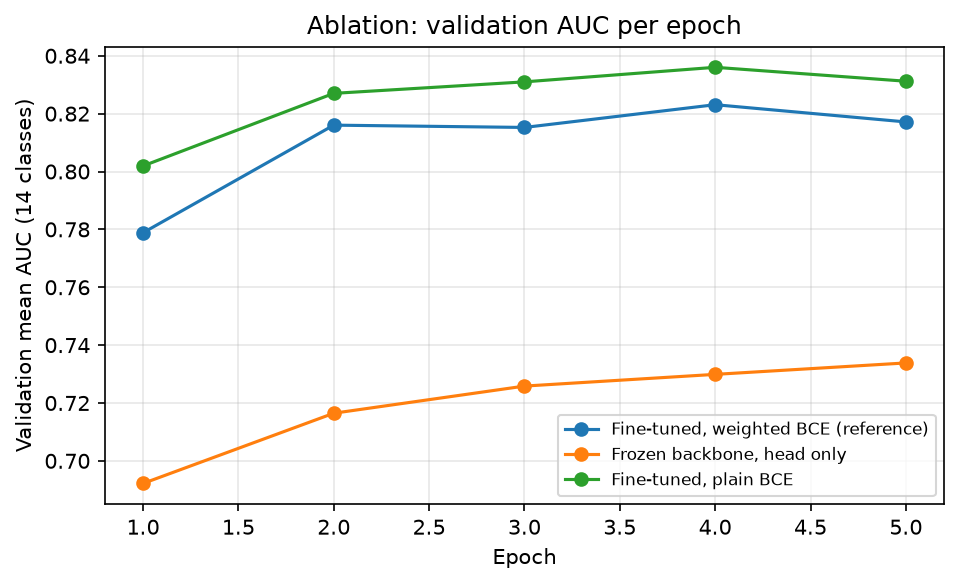
\includegraphics[height=9.5cm,width=0.75\textwidth,keepaspectratio]{ablation_curves.png}\end{center}}{}}{%
Results not available yet.}

\newpage
{\Large\bfseries 11. Training prevalence and loss weights}\par\vspace{0.5em}
\begin{center}\small\begin{tabular}{lrrrr}
\toprule
Disease & Train positives & Prevalence (\%) & \texttt{pos\_weight} & Test AUC \\
\midrule
Atelectasis & 7{,}003 & 9.47 & 9.6 & 0.751 \\
Cardiomegaly & 1{,}453 & 1.97 & 49.9 & 0.871 \\
Consolidation & 2{,}482 & 3.36 & 28.8 & 0.729 \\
Edema & 1{,}201 & 1.62 & 60.5 & 0.840 \\
Effusion & 7{,}415 & 10.03 & 9.0 & 0.816 \\
Emphysema & 1{,}274 & 1.72 & 57.0 & 0.909 \\
Fibrosis & 1{,}051 & 1.42 & 69.3 & 0.809 \\
Hernia & 113 & 0.15 & 653.1 & 0.933 \\
Infiltration & 11{,}853 & 16.04 & 5.2 & 0.693 \\
Mass & 3{,}452 & 4.67 & 20.4 & 0.792 \\
Nodule & 4{,}042 & 5.47 & 17.3 & 0.738 \\
Pleural Thickening & 1{,}870 & 2.53 & 38.5 & 0.766 \\
Pneumonia & 742 & 1.00 & 98.6 & 0.688 \\
Pneumothorax & 2{,}287 & 3.09 & 31.3 & 0.849 \\
\bottomrule
\end{tabular}
\end{center}

\newpage
{\Large\bfseries 12. Grad-CAM examples}\par
{\small\color{black!65} Original (left) and heatmap for the labelled disease (right). Confident test cases chosen for demonstration. Localisation is measured in slide 18.}\par\vspace{0.4em}
\begin{center}
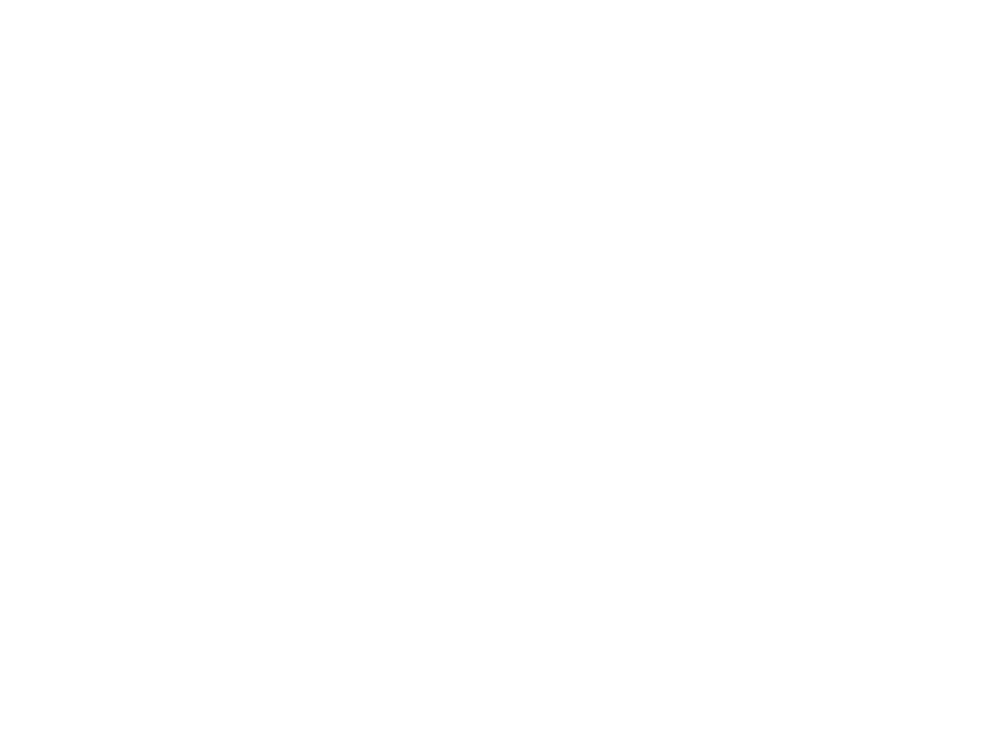
\includegraphics[width=0.82\textwidth]{gradcam_Cardiomegaly.png}\\[0.2em]
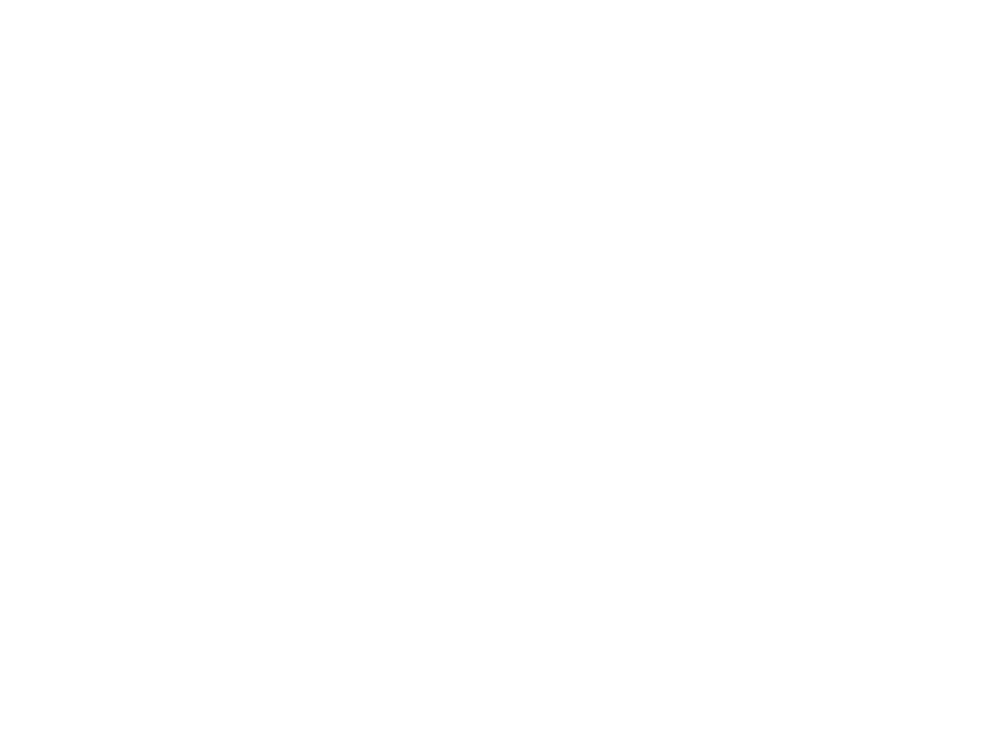
\includegraphics[width=0.82\textwidth]{gradcam_Effusion.png}\\[0.2em]
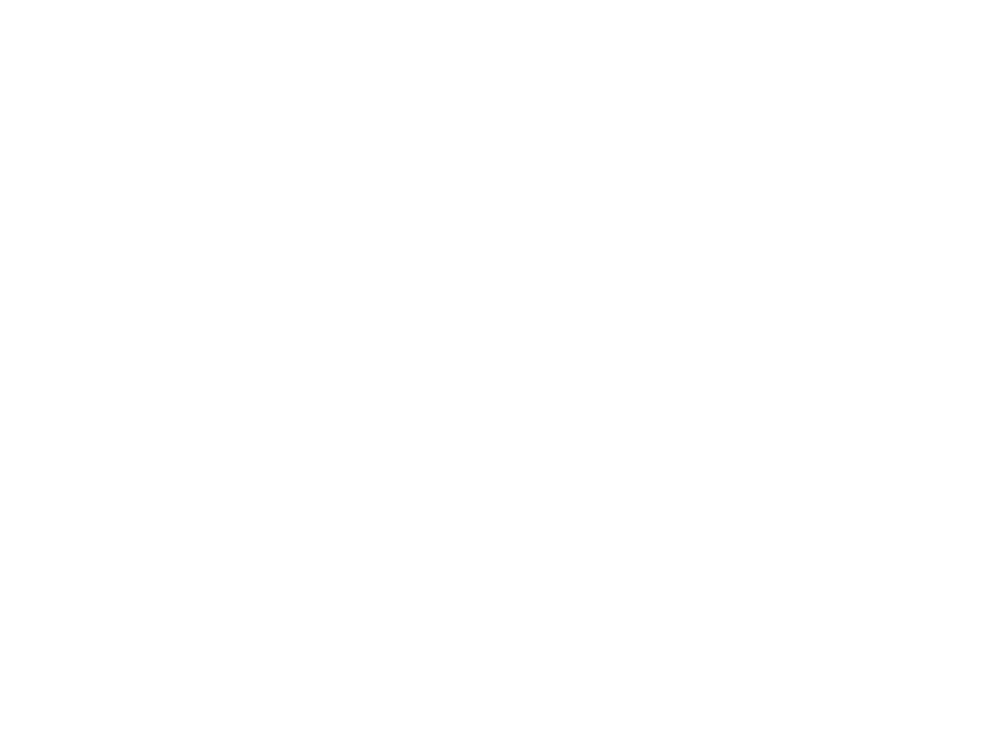
\includegraphics[width=0.82\textwidth]{gradcam_Emphysema.png}
\end{center}
\newpage
\begin{center}
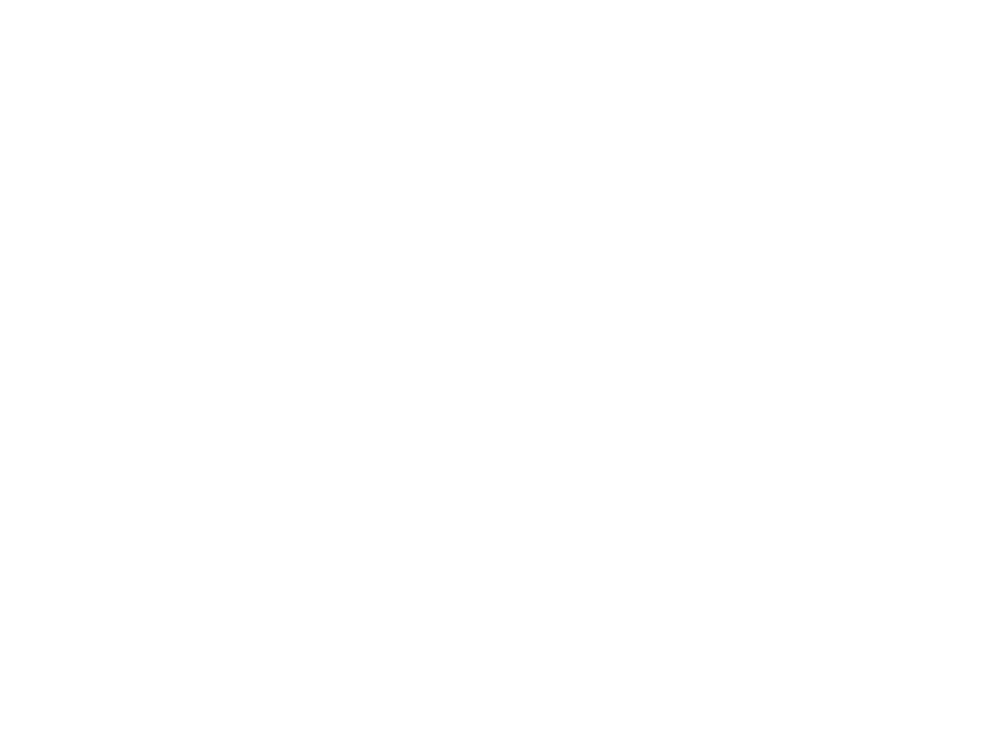
\includegraphics[width=0.82\textwidth]{gradcam_Pneumothorax.png}\\[0.2em]
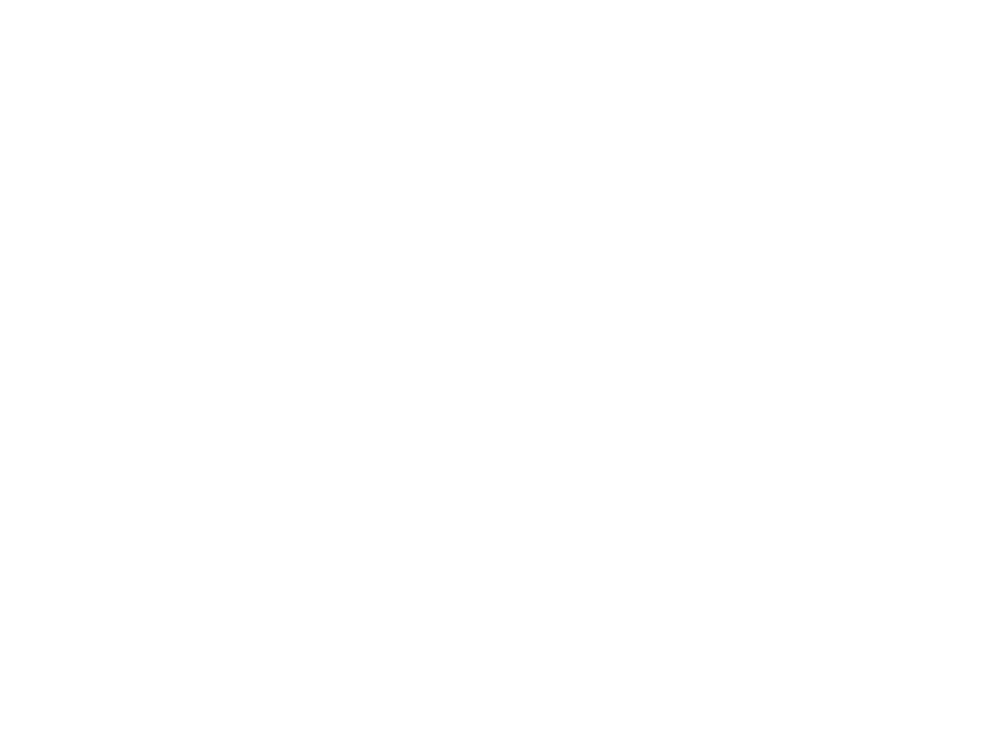
\includegraphics[width=0.82\textwidth]{gradcam_Edema.png}\\[0.2em]
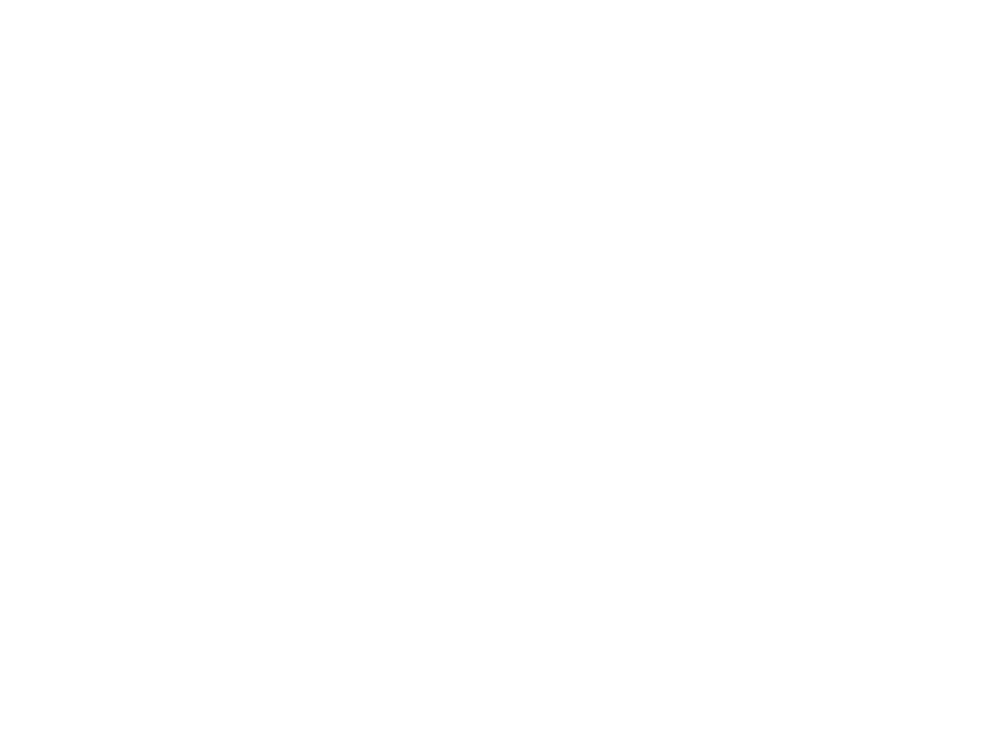
\includegraphics[width=0.82\textwidth]{gradcam_Mass.png}
\end{center}

\slide{13. The web app}{Pick an example or upload an X-ray: 14 probabilities, latency, Grad-CAM for any disease (screenshot).}{app_2_cardiomegaly.png}{16.2cm}
\slide{13b. The web app, other disease selected}{Any of the 14 diseases can be selected; heatmaps show where the model looked, not a diagnosis.}{app_3_effusion.png}{16.2cm}

% ---------------------------------------------------------------- after the first review
\slide{14. Same study, four architectures}{Fine-tuning matters for every network ($-0.09$ to $-0.16$ when frozen). Weighted BCE is lower on 3 of 4 (significant); EfficientNet-B0 not significant.}{grid_heatmap.png}{14cm}

\newpage
{\Large\bfseries 15. Seeds: is the loss effect real?}\par
{\small\color{black!65} DenseNet121 trained 3 times per loss. Every plain-BCE run beats every weighted run on test; the gap is about 4$\times$ the seed-to-seed spread.}\par\vspace{1.5em}
\begin{center}\large\begin{tabular}{lccc}
\toprule
DenseNet121 & Seeds & Val AUC (mean $\pm$ sd) & Test AUC (mean $\pm$ sd) \\
\midrule
Fine-tuned, plain BCE & 3 & 0.8331 $\pm$ 0.0020 & 0.8056 $\pm$ 0.0024 \\
Fine-tuned, weighted BCE & 3 & 0.8190 $\pm$ 0.0013 & 0.7968 $\pm$ 0.0009 \\
\bottomrule
\end{tabular}
\end{center}
\vspace{1em}
\begin{center}\small\resizebox{0.95\textwidth}{!}{\begin{tabular}{lccc}
\toprule
Architecture & Fine-tuned, plain BCE & Fine-tuned, weighted BCE & Frozen backbone, plain BCE \\
\midrule
DenseNet121 & 0.803 [0.796, 0.808] & 0.798 [0.791, 0.803] & 0.683 [0.675, 0.691] \\
ResNet50 & 0.798 [0.791, 0.804] & 0.792 [0.785, 0.798] & 0.664 [0.655, 0.672] \\
EfficientNet-B0 & 0.789 [0.782, 0.795] & 0.792 [0.785, 0.798] & 0.631 [0.623, 0.639] \\
ConvNeXt-Tiny & \textbf{0.809 [0.802, 0.814]} & \textbf{0.801 [0.793, 0.808]} & \textbf{0.721 [0.713, 0.728]} \\
\bottomrule
\end{tabular}
}\end{center}
\begin{center}\small Test mean AUC [95\% patient-bootstrap CI], seed 0.\end{center}

\newpage
{\Large\bfseries 16. Best model, ensemble and cost}\par
{\small\color{black!65} ConvNeXt-Tiny is best (0.809); its lead over DenseNet121 (0.006) is close to seed noise. The ensemble (0.816) beats every single model. EfficientNet-B0 is 6.5$\times$ faster.}\par\vspace{0.4em}
\begin{center}
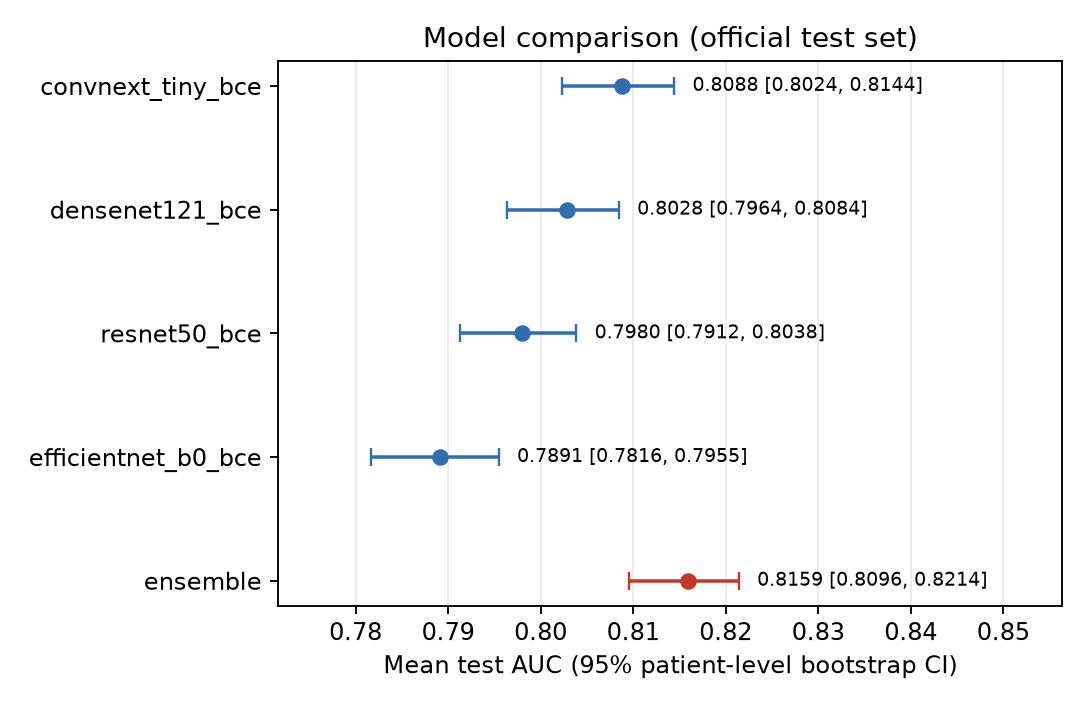
\includegraphics[height=11.5cm,width=0.49\textwidth,keepaspectratio]{forest_auc.png}\hfill
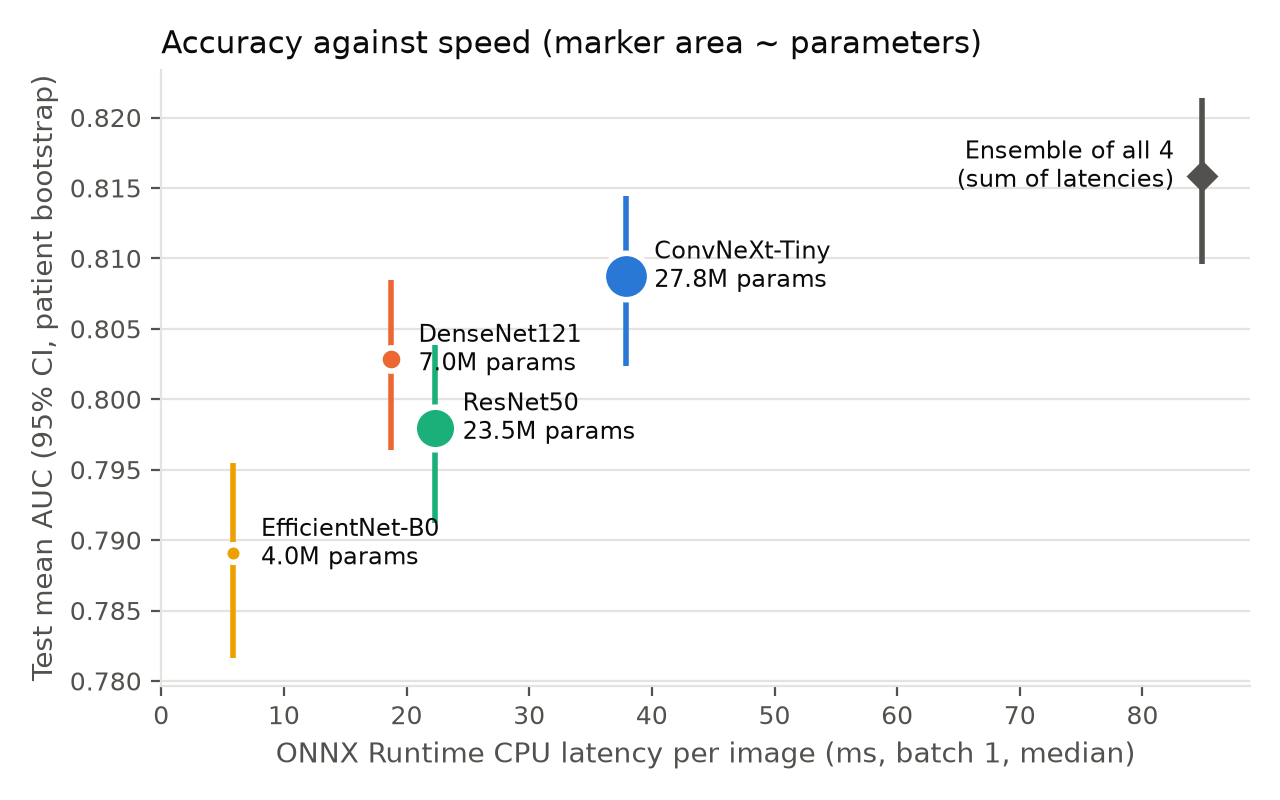
\includegraphics[height=11.5cm,width=0.49\textwidth,keepaspectratio]{pareto.png}
\end{center}

\slide{17. Calibration fixed}{Plain BCE is already calibrated (ECE 0.014), temperature scaling brings it to 0.007--0.013. Weighted BCE: ECE 0.33--0.36, which a temperature cannot fix (needs a bias).}{calibration_before_after.png}{15cm}

\newpage
{\Large\bfseries 18. Do the heatmaps point at the lesion?}\par
{\small\color{black!65} 984 radiologist boxes, none in our training split. ConvNeXt-Tiny points inside the box 44\% of the time, twice the image-centre baseline. Nodules are too small for a $7\times7$ map.}\par\vspace{0.4em}
\begin{center}
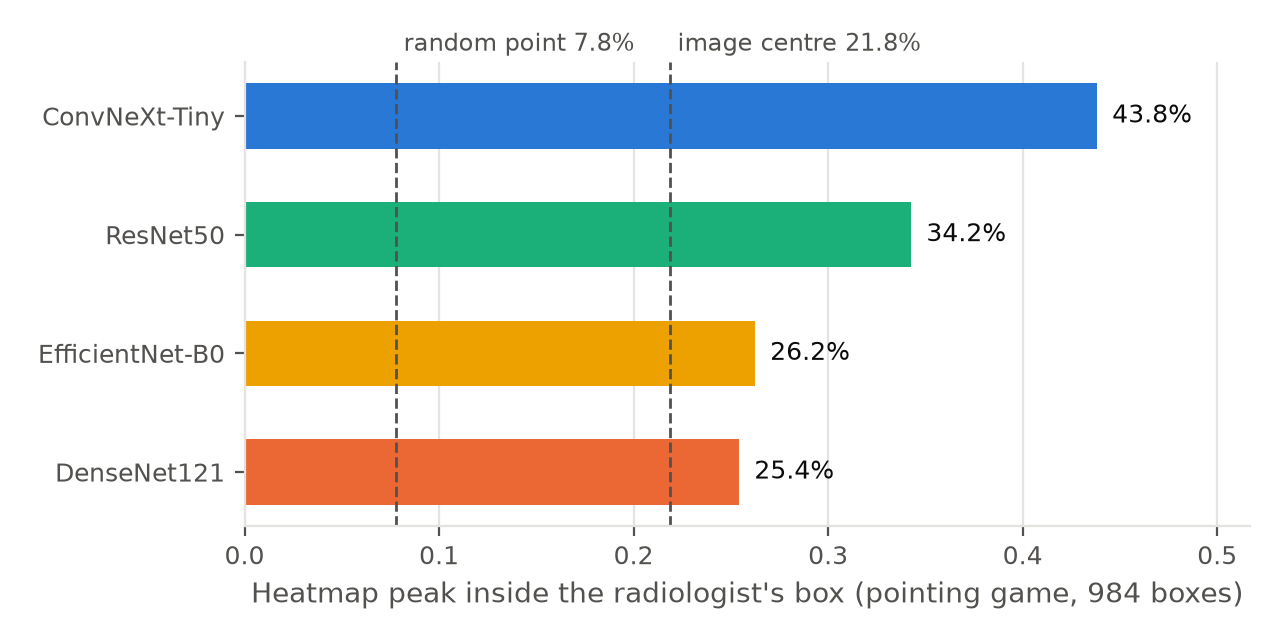
\includegraphics[height=6.6cm,width=0.49\textwidth,keepaspectratio]{localization_bars.png}\hfill
\begin{minipage}[b]{0.46\textwidth}\centering\small\resizebox{\textwidth}{!}{\begin{tabular}{lccc}
\toprule
Model & Pointing game (hit) & Energy in box & IoU (heat $\geq$ 0.5) \\
\midrule
ConvNeXt-Tiny & 0.438 & 0.299 & 0.178 \\
ResNet50 & 0.342 & 0.227 & 0.127 \\
EfficientNet-B0 & 0.262 & 0.117 & 0.135 \\
DenseNet121 & 0.254 & 0.176 & 0.145 \\
\midrule
Random point (baseline) & 0.078 & -- & -- \\
Image centre (baseline) & 0.218 & -- & -- \\
\bottomrule
\end{tabular}
}\vspace{2em}\end{minipage}\\[0.4em]
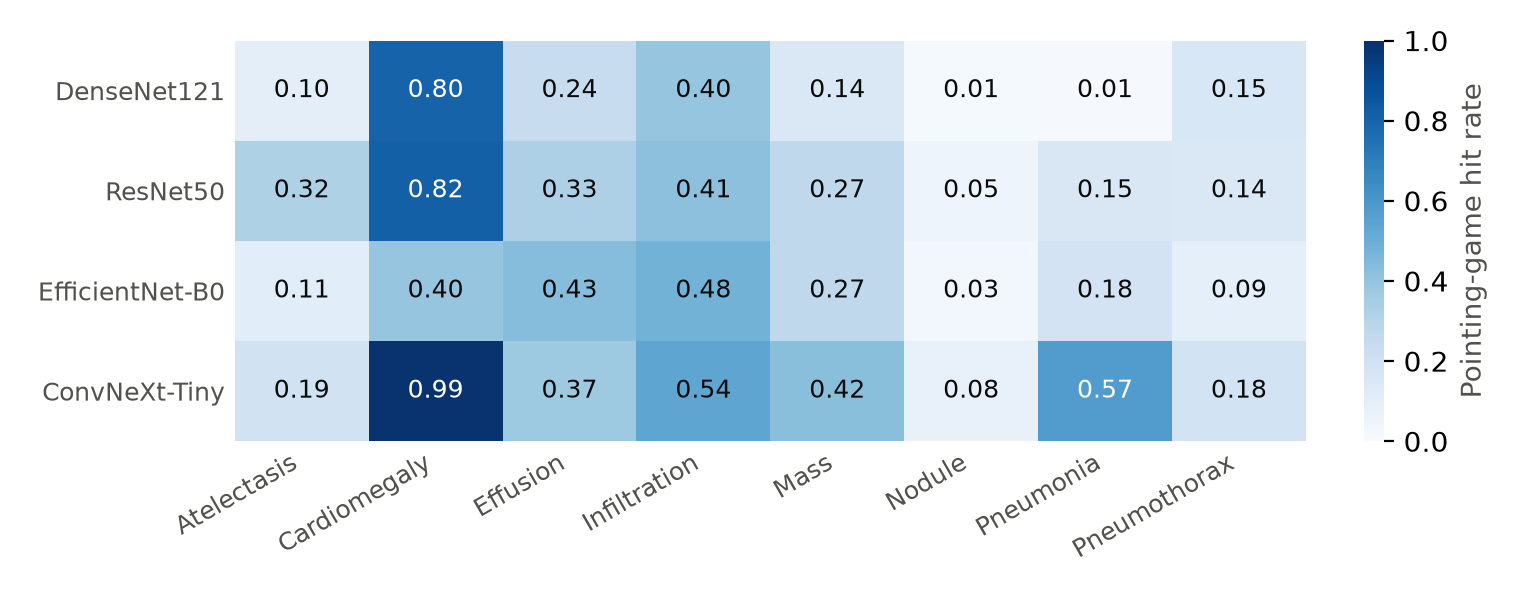
\includegraphics[height=6.4cm,width=0.85\textwidth,keepaspectratio]{localization_per_disease.png}
\end{center}

\slide{19. Subgroups}{No gap between men and women. Patients under 40 and bedside AP films are harder, for every architecture.}{subgroups.png}{14.5cm}

\slide{20. Compare models in the app}{Same X-ray through every model and the ensemble, running in Docker. Three heatmaps cover the heart; EfficientNet-B0 looks elsewhere.}{app_compare.jpg}{15.5cm}

\newpage
{\Large\bfseries 21. The role of Docker}\par
{\small\color{black!65} Docker delivers the trained models; it does not train them (training runs on Kaggle GPUs).}\par\vspace{2.5em}
\begin{center}\large
\setlength{\tabcolsep}{6pt}
\begin{tabular}{c c c c c}
\fbox{\begin{minipage}{0.15\textwidth}\centering Browser\\{\small React app}\end{minipage}}
& $\xrightarrow{\ \texttt{:8080}\ }$ &
\fbox{\begin{minipage}{0.22\textwidth}\centering \textbf{web} container\\{\small nginx: app + proxy \texttt{/api}}\\{\small 76\,MB}\end{minipage}}
& $\xrightarrow{\ \texttt{/api}\ }$ &
\fbox{\begin{minipage}{0.28\textwidth}\centering \textbf{api} container\\{\small FastAPI, ONNX Runtime, PyTorch}\\{\small 2.65\,GB, health-checked}\end{minipage}}\\[1em]
& & & & $\uparrow$ {\small read-only volume}\\[0.4em]
& & & &
\fbox{\begin{minipage}{0.28\textwidth}\centering \texttt{./models}\\{\small registry + 4 models (DVC)}\end{minipage}}
\end{tabular}
\end{center}
\vspace{2em}
\begin{itemize}\large
  \item \textbf{Same environment everywhere:} Python, PyTorch, ONNX Runtime versions frozen in the image.
  \item \textbf{Two services:} static app behind nginx, model server apart; one origin for the browser.
  \item \textbf{Weights are mounted, not baked in:} adding a model = edit \texttt{registry.json} + restart.
  \item \textbf{One command:} \texttt{docker compose up}; CI builds both images on every change.
\end{itemize}
\end{document}
